\documentclass[12pt]{article}

\usepackage{sbc-template}
\usepackage{graphicx,url}
\usepackage[utf8]{inputenc}
\usepackage[T1]{fontenc}
\usepackage[brazilian]{babel}
\usepackage{booktabs}
\usepackage[hidelinks]{hyperref}

% O sbc-template.sty (2017) registra, para uso com hyperref, uma redefinição
% de \@lbibitem que é executada no início do documento e, nas versões atuais
% do LaTeX, quebra o código do babel executado em seguida ("Undefined control
% sequence" em \begin{document}). A mesma redefinição é aplicada aqui, no
% preâmbulo, e o trecho original é removido.
\RemoveFromHook{begindocument/before}[sbc-template]
\makeatletter
\def\@lbibitem[#1]#2{%
  \@skiphyperreftrue
  \H@item[%
    \ifx\Hy@raisedlink\@empty
      \hyper@anchorstart{cite.#2\@extra@b@citeb}\hyper@anchorend
    \else
      \Hy@raisedlink{\hyper@anchorstart{cite.#2\@extra@b@citeb}\hyper@anchorend}%
    \fi
    \hfill]%
  \@skiphyperreffalse
  \if@filesw
    \begingroup
      \let\protect\noexpand
      \immediate\write\@auxout{\string\bibcite{#2}{#1}}%
    \endgroup
  \fi
  \ignorespaces}
\makeatother

% Gráficos copiados da pasta figures/ do repositório, onde são gerados por
% scripts/analyze.py e scripts/compare-levels.py.
\graphicspath{{figures/}}

% Espaço entre figuras e texto um pouco menor que o padrão, para caber nas
% 5 páginas.
\setlength{\textfloatsep}{10pt plus 2pt minus 2pt}
\setlength{\floatsep}{8pt plus 2pt minus 2pt}
\setlength{\intextsep}{8pt plus 2pt minus 2pt}

\newcommand{\repo}{https://github.com/EduardoFerreiraB/Redes-Moveis}

\sloppy

\title{Mobilidade e Área no Desempenho de AODV, OLSR e DSDV\\
em MANETs com Aproximação de Perdas Ambientais}

\author{Eduardo Ferreira de Brito Matos\inst{1}, Pedro Américo Rocha\inst{1},
  Thiago Ferreira\inst{1}}
\address{Instituto Federal de Educação, Ciência e Tecnologia de Goiás (IFG)\\
  Câmpus Inhumas -- Inhumas, GO -- Brasil
  \email{eduardoferreirabmatos@gmail.com, pedroamericorocha@gmail.com,}\\
  \footnotesize\texttt{thiagoferreira2004f@gmail.com}
}

\begin{document}
\maketitle
% Gerado por scripts/prepare-article.py; não editar números manualmente.
\newcommand{\ResultAbstract}{At 20 m/s in the baseline area, mean PDR was 66.3\% for AODV, 32.8\% for OLSR and 36.4\% for DSDV.}
\newcommand{\ResultResumo}{A 20 m/s na área-base, o PDR médio foi 66,3\% no AODV, 32,8\% no OLSR e 36,4\% no DSDV.}
\newcommand{\ResultConclusao}{No cenário-base, o aumento de 1 para 20 m/s reduziu a entrega dos três protocolos. AODV obteve o maior PDR médio a 20 m/s, com maior atraso que os proativos. Nessa velocidade, ampliar a área reduziu a entrega de todos os protocolos. A tendência com a velocidade, contudo, não é uniforme entre áreas. }

\begin{abstract}
This paper evaluates AODV, OLSR and DSDV in a 20-node MANET using ns-3.48.
Node speed is the main factor (1, 5, 10 and 20 m/s), and square side length
is the additional factor (300, 500 and 700 m). The IEEE 802.11b radio uses a
fixed 16 dBm power at 2.412 GHz. A log-distance model with exponent 2.7
approximates average environmental attenuation, without explicit obstacles
or terrain. The 720 simulations use 20 runs per configuration and report PDR,
throughput, delay and jitter. \ResultAbstract{}
The findings apply to the assumed channel and mobility model, without field calibration.
\textbf{Keywords:} MANET; mobility; routing; ns-3.
\end{abstract}

\begin{resumo}
Este artigo avalia AODV, OLSR e DSDV em uma MANET de 20 nós no ns-3.48.
A velocidade é o fator principal (1, 5, 10 e 20 m/s), e o lado da área
quadrada é o fator adicional (300, 500 e 700 m). O rádio IEEE 802.11b opera
com 16 dBm fixos em 2,412 GHz. O modelo log-distance com expoente 2,7
aproxima a atenuação ambiental média, sem obstáculos ou relevo explícitos.
As 720 simulações usam 20 runs por configuração e medem PDR, vazão, atraso
e jitter. \ResultResumo{}
Os resultados são condicionados aos modelos adotados, sem calibração de campo.
\textbf{Palavras-chave:} MANET; mobilidade; roteamento; ns-3.
\end{resumo}

\section{Introdução}
Em uma MANET, dispositivos móveis comunicam-se sem infraestrutura fixa
e encaminham pacotes por múltiplos saltos. Este trabalho investiga como
a velocidade afeta AODV, OLSR e DSDV e se essa tendência muda quando a mesma
quantidade de nós ocupa áreas diferentes.

A investigação adicional foi reformulada: a área substitui a variação da
potência. Mantêm-se frequência e potência fixas para comparar os protocolos
sob um mesmo rádio. A propagação deixa de assumir espaço livre e passa a
incluir uma aproximação de perda ambiental média. Essa escolha torna as
hipóteses mais explícitas, mas não equivale a reproduzir um local real.

\section{Fundamentação Teórica}
O \textbf{AODV} descobre rotas sob demanda, usando pedidos RREQ, respostas
RREP e notificações de quebra; pacotes podem aguardar a descoberta em
fila~\cite{rfc3561}. O \textbf{OLSR} mantém rotas proativamente, com mensagens
HELLO e TC e retransmissores multiponto para divulgar a
topologia~\cite{rfc3626}. O \textbf{DSDV} mantém tabelas de distância e usa
números de sequência para distinguir atualizações e evitar
laços~\cite{perkins1994}.

Terreno plano e propagação em espaço livre são conceitos diferentes: uma
superfície plana pode conter vegetação e edificações. Já relevo envolve
variação de elevação. Um modelo de perda média por distância não descreve
geometricamente nenhum desses obstáculos. Portanto, a presente investigação
é uma comparação controlada sob atenuação agregada, não uma previsão de
cobertura urbana ou de terreno tridimensional.

\section{Metodologia}
Utilizou-se ns-3.48, commit \texttt{d2add90b452d}, com a configuração da
Tabela~\ref{tab:cenario}. A matriz-base permanece com 500 $\times$ 500 m,
três protocolos e quatro velocidades. A variável adicional acrescenta
300 $\times$ 300 e 700 $\times$ 700 m. São 3 áreas $\times$ 3 protocolos
$\times$ 4 velocidades $\times$ 20 runs = 720 execuções novas.

\begin{table}[ht]
\centering
\caption{Parâmetros da campanha revisada}
\label{tab:cenario}
\small
\begin{tabular}{ll}
\toprule
Parâmetro & Valor \\
\midrule
Nós / áreas & 20 / lados de 300, 500 e 700 m \\
Rádio & IEEE 802.11b ad hoc, DSSS a 11 Mb/s, taxa fixa \\
Canal / potência & Canal 1, 2,412 GHz, 22 MHz / 16 dBm fixos \\
Antenas & Ganhos TX/RX de 0 dB; altura comum de 1,5 m \\
Propagação & Log-distance: $n=2{,}7$, $d_0=1$ m, $L_0=40{,}0953$ dB \\
Mobilidade & Random Waypoint; pausa 0 s; 1, 5, 10 e 20 m/s \\
Tráfego & 4 fluxos UDP; 32768 bit/s por fluxo; 1024 bytes \\
Duração & 120 s; cada fonte ativa por 90 s; início em [20,21) s \\
Aleatoriedade & Seed 1; runs 1 a 20; trajetórias pareadas por protocolo \\
\bottomrule
\end{tabular}
\end{table}

\subsection{Rádio e aproximação ambiental}
O PHY foi configurado explicitamente no canal 1. Na implementação anterior,
o modelo Friis conservava a frequência padrão de 5,15 GHz do ns-3, incompatível
com o canal 802.11b. Essa inconsistência foi corrigida; os alcances e os
resultados anteriores não são reutilizados nesta análise.
Escolheu-se 16 dBm (aproximadamente 39,8 mW), dentro da faixa de 13--20 dBm
informada pelo grupo para o equipamento de interesse. Essa faixa é uma
restrição de projeto, não um limite universal do IEEE 802.11b; sem ficha
técnica específica não se alega validação do hardware. Há somente um nível
de potência, sem ajuste adaptativo nem mudança de frequência durante as runs.

Emprega-se \texttt{LogDistancePropagationLossModel}~\cite{ns3propagation}:
\begin{equation}
L(d)=L_0+10n\log_{10}(d/d_0),\qquad
L_0=20\log_{10}(4\pi f d_0/c).
\end{equation}
Para $d>d_0$, $L(d)$ é a perda em dB, $d$ a distância em metros,
$d_0=1$ m, $f=2{,}412$ GHz e $c$ a velocidade da luz. Resulta
$L_0=40{,}0953$ dB. O expoente $n=2{,}7$ foi adotado como hipótese de perda
superior ao espaço livre ($n=2$), sem ajuste aos resultados de PDR.
Não é um valor medido ou universal para árvores e prédios. O mesmo expoente
é mantido em todas as áreas para evitar confundir efeitos de área e canal.

O modelo é determinístico e homogêneo: não inclui paredes, árvores, sombras
espacialmente correlacionadas, desvanecimento aleatório ou difração por
relevo. A coordenada $z=1{,}5$ m é constante; não cria topografia nem
efeito de altura no modelo adotado. Para $d\leq1$ m, a implementação do
ns-3.48 mantém a perda em $L_0$, uma aproximação de curta distância.
Não se interpreta, portanto, a atenuação adicional como geometria explícita.

\subsection{Controle experimental e métricas}
Mantêm-se 20 nós nas três áreas, correspondendo a 222,2, 80,0 e 40,8
nós/km$^2$. Variar a área muda simultaneamente a densidade, as distâncias e
os tempos de travessia; esses mecanismos não são isolados. Random Waypoint
usa posições iniciais uniformes, destinos aleatórios e velocidade constante.
Streams fixos garantem trajetórias e inícios de tráfego iguais entre
protocolos na mesma área, velocidade e run; entre áreas as trajetórias
físicas diferem. Os fluxos vão do nó $i+4$ ao nó $i$, para $i=0,\ldots,3$.

Os inícios são sorteados em [20,21) s para reduzir sincronização dos pedidos
ARP. O \texttt{ArpCache::DeadTimeout} é 1 s em todos os protocolos, permitindo
retentar vizinhos móveis; o \texttt{MaxPerHopDelay} do FlowMonitor é 120 s
para registrar entregas que aguardaram rota. As fontes terminam até 111 s,
deixando ao menos 9 s para drenagem, que pode não esvaziar todas as filas.

Consideram-se apenas os dados UDP destinados à porta 9. O denominador do
\textbf{PDR} é a demanda nominal de 1436 pacotes (359 oportunidades por
fluxo em 90 s), incluindo demanda não atendida quando a aplicação não
consegue enviar por falta de rota; não é o número de objetos efetivamente
gerados pelo OnOff. Envios efetivos são registrados separadamente. A
\textbf{vazão} é $8B_{rx}/90$ s, com bytes de aplicação recebidos até 120 s,
inclusive durante a drenagem. O \textbf{atraso} é
$\sum delaySum/\sum rxPackets$, a partir da observação IP; o
\textbf{jitter} é $\sum jitterSum/\sum\max(rxPackets-1,0)$, por fluxo,
usando FlowMonitor~\cite{ns3flow}. Ambos são condicionados à entrega;
sem amostras válidas, são indefinidos. Saltos médios são
$1+\sum timesForwarded/\sum rxPackets$ dos pacotes entregues.

Calculam-se média, desvio-padrão, mínimo, máximo e IC de 95\% com distribuição
$t$ entre runs independentes. Barras de erro não são um teste de significância
entre protocolos. Os CSVs registram os parâmetros do rádio e do ambiente,
evitando misturar resultados de configurações diferentes.

\subsection{Reprodutibilidade}
O código, os comandos por run, os CSVs e os scripts de análise compõem a
entrega revisada. O endereço do projeto é:
\begin{center}
\textbf{\url{\repo}}
\end{center}
O README descreve os comandos de execução, análise e geração do artigo.
A revisão está identificada como 19/11/2026 nos arquivos da entrega.

\section{Resultados e Discussão}

Na área-base de 500 $\times$ 500 m (Figura~\ref{fig:pdr}), o PDR médio cai
de 85,2\%, 81,0\% e 78,6\% a 1 m/s para 66,3\%, 32,8\% e 36,4\% a 20 m/s, respectivamente para AODV,
OLSR e DSDV. A vazão acompanha a entrega porque a demanda é fixa.
O comportamento é compatível com a dificuldade de manter rotas sob mobilidade,
mas as métricas agregadas não separam perdas por ausência de caminhos,
desatualização de rotas e contenção no canal.

\begin{figure}[ht]
\centering
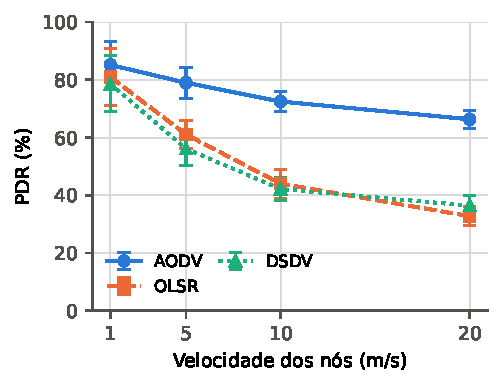
\includegraphics[width=.42\textwidth]{area-500m/pdr-vs-velocidade}
\hfill
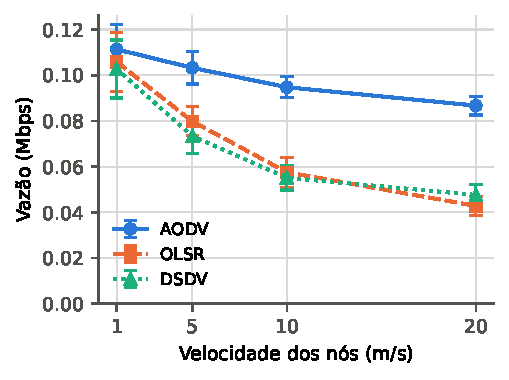
\includegraphics[width=.42\textwidth]{area-500m/vazao-vs-velocidade}
\caption{PDR e vazão no cenário-base (média e IC de 95\%, 20 runs).}
\label{fig:pdr}
\end{figure}

O atraso médio do AODV passa de 14,8 para 137,4 ms entre 1 e
20 m/s. A 20 m/s, OLSR e DSDV apresentam 15,7 e 12,0 ms, com menor entrega.
Atraso e jitter (Figura~\ref{fig:atraso}) devem ser lidos com o PDR:
os pacotes perdidos não entram nas médias e o descarte de trajetos difíceis
pode favorecer artificialmente a leitura de latência. Não se conclui
superioridade geral de um protocolo a partir de uma única métrica.

\begin{figure}[ht]
\centering
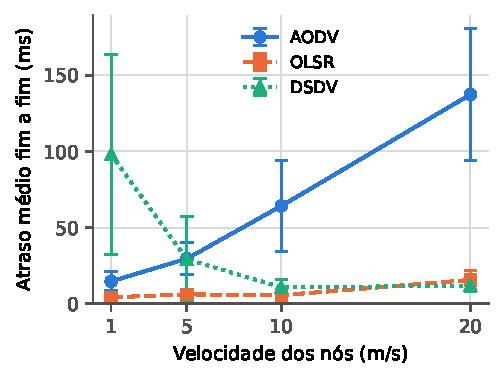
\includegraphics[width=.42\textwidth]{area-500m/atraso-vs-velocidade}
\hfill
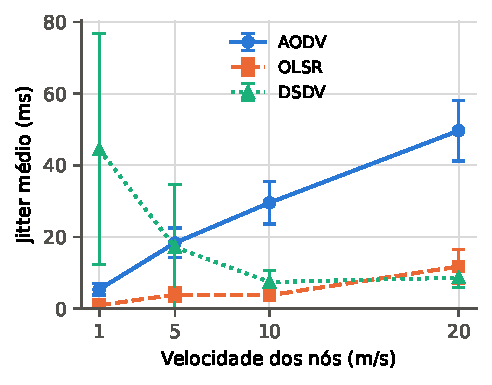
\includegraphics[width=.42\textwidth]{area-500m/jitter-vs-velocidade}
\caption{Atraso e jitter no cenário-base (média e IC de 95\%).}
\label{fig:atraso}
\end{figure}

A Figura~\ref{fig:comparativo} resume o base a 10 m/s: os PDRs são
72,5\%, 44,0\% e 42,2\%, na ordem AODV, OLSR e DSDV. As médias entre runs dos saltos dos
pacotes entregues são 2,3; 1,7; 1,7, confirmando encaminhamento por múltiplos
saltos em parte das entregas. Isso não estima a conectividade dos pares
que não entregaram pacotes.

\begin{figure}[ht]
\centering
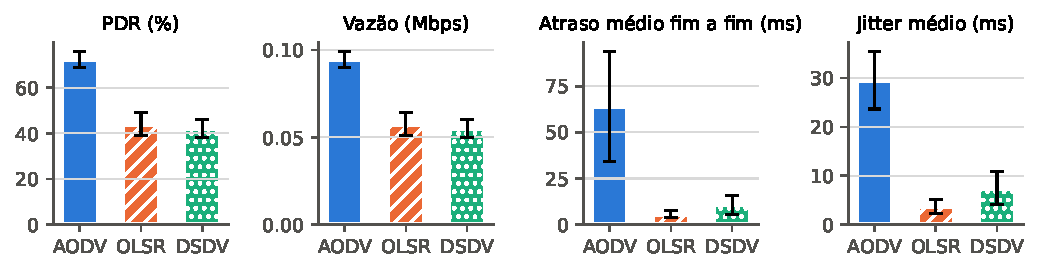
\includegraphics[width=.92\textwidth]{area-500m/comparativo-10ms}
\caption{Comparação dos protocolos a 10 m/s no base (média e IC de 95\%).}
\label{fig:comparativo}
\end{figure}

A variável adicional altera a entrega sem modificar o rádio
(Figura~\ref{fig:area}). A 20 m/s, o PDR médio em 300 $\times$ 300 m é
87,2\%, 67,0\% e 67,7\%, enquanto em 700 $\times$ 700 m é 37,3\%, 14,4\% e 18,0\%, na mesma ordem
de protocolos. A redução de densidade e o aumento de distâncias são
compatíveis com essa degradação. Não se atribui o resultado a prédios ou
árvores específicos: o ambiente é representado apenas pelo expoente fixo.
Os ICs mostram a dispersão entre runs; não se realizou teste de hipótese
para declarar diferenças estatisticamente significativas entre protocolos.
Em 700 $\times$ 700 m, o PDR médio do AODV sobe de 35,5\% a 1 m/s
para 52,2\% a 5 m/s, antes de cair: a tendência do base não é universal.
O possível efeito de novos encontros e do transiente de mobilidade não foi
isolado por medidas de conectividade temporal.

\begin{figure}[ht]
\centering
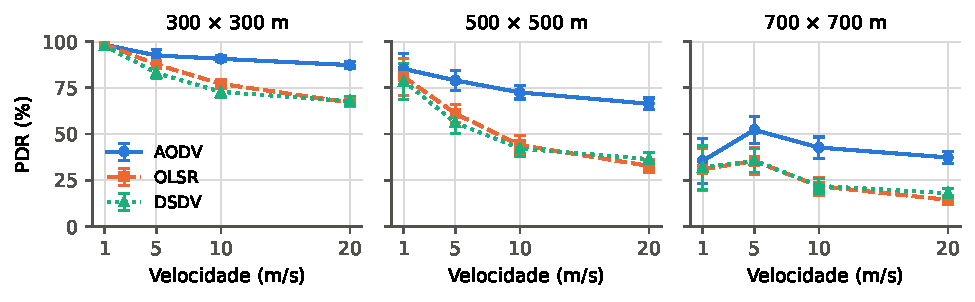
\includegraphics[width=.9\textwidth]{area/pdr-por-area}
\caption{PDR por velocidade nas três áreas, com rádio e canal de propagação
fixos (média e IC de 95\%).}
\label{fig:area}
\end{figure}


\section{Conclusão}
\ResultConclusao{}
Os resultados limitam-se a 20 nós, tráfego leve e expoente 2,7. O aquecimento
de 20 s não garante estacionariedade do Random Waypoint. Sem calibração,
ruas, obstáculos, relevo ou interferência externa explícitos, não se prevê
cobertura real. Estudos futuros devem medir o canal, testar sensibilidade
ao expoente e combinar mobilidade e obstruções compatíveis com um mapa.

\bibliographystyle{sbc}
\bibliography{referencias}
\end{document}
